\documentclass{book}
\usepackage[a4paper,top=2.5cm,bottom=2.5cm,left=2.5cm,right=2.5cm]{geometry}
\usepackage{makeidx}
\usepackage{natbib}
\usepackage{graphicx}
\usepackage{multicol}
\usepackage{float}
\usepackage{listings}
\usepackage{color}
\usepackage{ifthen}
\usepackage[table]{xcolor}
\usepackage{textcomp}
\usepackage{alltt}
\usepackage{ifpdf}
\ifpdf
\usepackage[pdftex,
            pagebackref=true,
            colorlinks=true,
            linkcolor=blue,
            unicode
           ]{hyperref}
\else
\usepackage[ps2pdf,
            pagebackref=true,
            colorlinks=true,
            linkcolor=blue,
            unicode
           ]{hyperref}
\usepackage{pspicture}
\fi
\usepackage[utf8]{inputenc}
\usepackage{mathptmx}
\usepackage[scaled=.90]{helvet}
\usepackage{courier}
\usepackage{sectsty}
\usepackage{amssymb}
\usepackage[titles]{tocloft}
\usepackage{doxygen}
\lstset{language=C++,inputencoding=utf8,basicstyle=\footnotesize,breaklines=true,breakatwhitespace=true,tabsize=4,numbers=left }
\makeindex
\setcounter{tocdepth}{3}
\renewcommand{\footrulewidth}{0.4pt}
\renewcommand{\familydefault}{\sfdefault}
\hfuzz=15pt
\setlength{\emergencystretch}{15pt}
\hbadness=750
\tolerance=750
\begin{document}
\hypersetup{pageanchor=false,citecolor=blue}
\begin{titlepage}
\vspace*{7cm}
\begin{center}
{\Large Calculatrice\-Simple \\[1ex]\large 1.\-0 }\\
\vspace*{1cm}
{\large Generated by Doxygen 1.8.2}\\
\vspace*{0.5cm}
{\small Thu Sep 27 2012 11:58:27}\\
\end{center}
\end{titlepage}
\clearemptydoublepage
\pagenumbering{roman}
\tableofcontents
\clearemptydoublepage
\pagenumbering{arabic}
\hypersetup{pageanchor=true,citecolor=blue}
\chapter{Namespace Index}
\section{Packages}
Here are the packages with brief descriptions (if available)\-:\begin{DoxyCompactList}
\item\contentsline{section}{\hyperlink{namespacecom}{com} }{\pageref{namespacecom}}{}
\item\contentsline{section}{\hyperlink{namespacecom_1_1example}{com.\-example} }{\pageref{namespacecom_1_1example}}{}
\item\contentsline{section}{\hyperlink{namespacecom_1_1example_1_1calculatrice}{com.\-example.\-calculatrice} }{\pageref{namespacecom_1_1example_1_1calculatrice}}{}
\end{DoxyCompactList}

\chapter{Hierarchical Index}
\section{Class Hierarchy}
This inheritance list is sorted roughly, but not completely, alphabetically\-:\begin{DoxyCompactList}
\item Activity\begin{DoxyCompactList}
\item \contentsline{section}{com.\-example.\-calculatrice.\-Calculatrice}{\pageref{classcom_1_1example_1_1calculatrice_1_1_calculatrice}}{}
\end{DoxyCompactList}
\end{DoxyCompactList}

\chapter{Class Index}
\section{Class List}
Here are the classes, structs, unions and interfaces with brief descriptions\-:\begin{DoxyCompactList}
\item\contentsline{section}{\hyperlink{classcom_1_1example_1_1calculatrice_1_1_calculatrice}{com.\-example.\-calculatrice.\-Calculatrice} }{\pageref{classcom_1_1example_1_1calculatrice_1_1_calculatrice}}{}
\end{DoxyCompactList}

\chapter{File Index}
\section{File List}
Here is a list of all files with brief descriptions\-:\begin{DoxyCompactList}
\item\contentsline{section}{C\-:/\-Users/\-Rouinsard/\-Java/\-Calculatrice/src/com/example/calculatrice/\hyperlink{_calculatrice_8java}{Calculatrice.\-java} }{\pageref{_calculatrice_8java}}{}
\end{DoxyCompactList}

\chapter{Namespace Documentation}
\hypertarget{namespacecom}{\section{Package com}
\label{namespacecom}\index{com@{com}}
}
\subsection*{Packages}
\begin{DoxyCompactItemize}
\item 
package \hyperlink{namespacecom_1_1example}{example}
\end{DoxyCompactItemize}

\hypertarget{namespacecom_1_1example}{\section{Package com.\-example}
\label{namespacecom_1_1example}\index{com.\-example@{com.\-example}}
}
\subsection*{Packages}
\begin{DoxyCompactItemize}
\item 
package \hyperlink{namespacecom_1_1example_1_1calculatrice}{calculatrice}
\end{DoxyCompactItemize}

\hypertarget{namespacecom_1_1example_1_1calculatrice}{\section{Package com.\-example.\-calculatrice}
\label{namespacecom_1_1example_1_1calculatrice}\index{com.\-example.\-calculatrice@{com.\-example.\-calculatrice}}
}
\subsection*{Classes}
\begin{DoxyCompactItemize}
\item 
class \hyperlink{classcom_1_1example_1_1calculatrice_1_1_calculatrice}{Calculatrice}
\end{DoxyCompactItemize}

\chapter{Class Documentation}
\hypertarget{classcom_1_1example_1_1calculatrice_1_1_calculatrice}{\section{com.\-example.\-calculatrice.\-Calculatrice Class Reference}
\label{classcom_1_1example_1_1calculatrice_1_1_calculatrice}\index{com.\-example.\-calculatrice.\-Calculatrice@{com.\-example.\-calculatrice.\-Calculatrice}}
}
Inheritance diagram for com.\-example.\-calculatrice.\-Calculatrice\-:\begin{figure}[H]
\begin{center}
\leavevmode
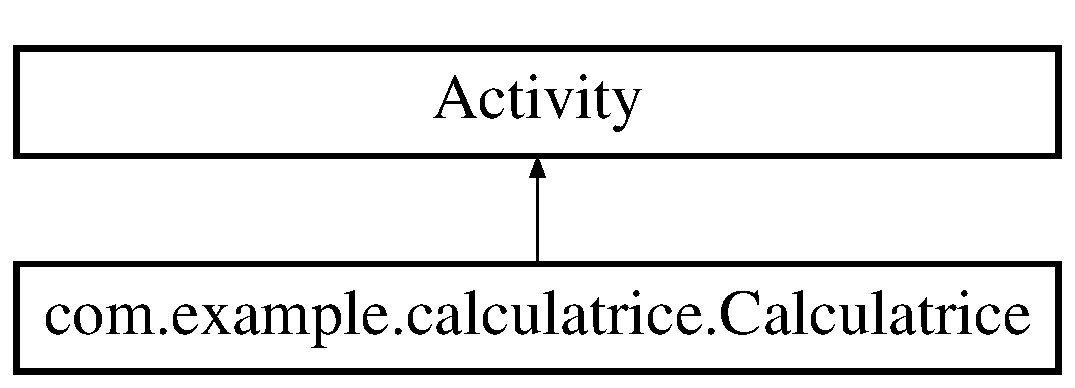
\includegraphics[height=2.000000cm]{classcom_1_1example_1_1calculatrice_1_1_calculatrice}
\end{center}
\end{figure}
\subsection*{Public Member Functions}
\begin{DoxyCompactItemize}
\item 
void \hyperlink{classcom_1_1example_1_1calculatrice_1_1_calculatrice_a522787a430f3b8375904dab26c4ab221}{on\-Create} (Bundle saved\-Instance\-State)
\begin{DoxyCompactList}\small\item\em sert a contenir le type d'operations a effectuer ==$>$ Description breve. \end{DoxyCompactList}\item 
boolean \hyperlink{classcom_1_1example_1_1calculatrice_1_1_calculatrice_a7f4f3e3f874d743a3e103d3798b60626}{on\-Create\-Options\-Menu} (Menu menu)
\item 
void \hyperlink{classcom_1_1example_1_1calculatrice_1_1_calculatrice_a451f694a60dcdddcfe450ad1abee159b}{addition} (View v)
\begin{DoxyCompactList}\small\item\em La fonction addition permet de faire une addition lors du clique sur \char`\"{}+\char`\"{} ==$>$ Description breve. \end{DoxyCompactList}\item 
void \hyperlink{classcom_1_1example_1_1calculatrice_1_1_calculatrice_a8e3dde2e6f1f65eaea278786e9b2a06d}{soustraction} (View v)
\begin{DoxyCompactList}\small\item\em La fonction soustraction permet de faire une soustraction lors du clique sur \char`\"{}-\/\char`\"{} ==$>$ Description breve. \end{DoxyCompactList}\item 
void \hyperlink{classcom_1_1example_1_1calculatrice_1_1_calculatrice_ae48705eb7153e48a9eada2a7c0c012fe}{multiplication} (View v)
\begin{DoxyCompactList}\small\item\em La fonction multiplication permet de faire une multiplication lors du clique sur \char`\"{}$\ast$\char`\"{} ==$>$ Description breve. \end{DoxyCompactList}\item 
void \hyperlink{classcom_1_1example_1_1calculatrice_1_1_calculatrice_a653a4d58c9076b6bdeb360a2d32042f3}{division} (View v)
\begin{DoxyCompactList}\small\item\em La fonction division permet de faire une division lors du clique sur \char`\"{}/\char`\"{} ==$>$ Description breve. \end{DoxyCompactList}\item 
void \hyperlink{classcom_1_1example_1_1calculatrice_1_1_calculatrice_ae481f686c7dbc697992ad7d84762af30}{resultat} (View v)
\begin{DoxyCompactList}\small\item\em La fonction resultats permet de faire le calcul lors du clique sur \char`\"{}=\char`\"{}, la fonction effectue le calcul puis l'affiche dans un Text\-View ==$>$ Description breve. \end{DoxyCompactList}\end{DoxyCompactItemize}


\subsection{Detailed Description}


Definition at line 11 of file Calculatrice.\-java.



\subsection{Member Function Documentation}
\hypertarget{classcom_1_1example_1_1calculatrice_1_1_calculatrice_a451f694a60dcdddcfe450ad1abee159b}{\index{com\-::example\-::calculatrice\-::\-Calculatrice@{com\-::example\-::calculatrice\-::\-Calculatrice}!addition@{addition}}
\index{addition@{addition}!com::example::calculatrice::Calculatrice@{com\-::example\-::calculatrice\-::\-Calculatrice}}
\subsubsection[{addition}]{\setlength{\rightskip}{0pt plus 5cm}void com.\-example.\-calculatrice.\-Calculatrice.\-addition (
\begin{DoxyParamCaption}
\item[{View}]{v}
\end{DoxyParamCaption}
)}}\label{classcom_1_1example_1_1calculatrice_1_1_calculatrice_a451f694a60dcdddcfe450ad1abee159b}


La fonction addition permet de faire une addition lors du clique sur \char`\"{}+\char`\"{} ==$>$ Description breve. 


\begin{DoxyParams}{Parameters}
{\em v} & La vue Android \\
\hline
\end{DoxyParams}


Definition at line 27 of file Calculatrice.\-java.

\hypertarget{classcom_1_1example_1_1calculatrice_1_1_calculatrice_a653a4d58c9076b6bdeb360a2d32042f3}{\index{com\-::example\-::calculatrice\-::\-Calculatrice@{com\-::example\-::calculatrice\-::\-Calculatrice}!division@{division}}
\index{division@{division}!com::example::calculatrice::Calculatrice@{com\-::example\-::calculatrice\-::\-Calculatrice}}
\subsubsection[{division}]{\setlength{\rightskip}{0pt plus 5cm}void com.\-example.\-calculatrice.\-Calculatrice.\-division (
\begin{DoxyParamCaption}
\item[{View}]{v}
\end{DoxyParamCaption}
)}}\label{classcom_1_1example_1_1calculatrice_1_1_calculatrice_a653a4d58c9076b6bdeb360a2d32042f3}


La fonction division permet de faire une division lors du clique sur \char`\"{}/\char`\"{} ==$>$ Description breve. 


\begin{DoxyParams}{Parameters}
{\em v} & La vue Android \\
\hline
\end{DoxyParams}


Definition at line 42 of file Calculatrice.\-java.

\hypertarget{classcom_1_1example_1_1calculatrice_1_1_calculatrice_ae48705eb7153e48a9eada2a7c0c012fe}{\index{com\-::example\-::calculatrice\-::\-Calculatrice@{com\-::example\-::calculatrice\-::\-Calculatrice}!multiplication@{multiplication}}
\index{multiplication@{multiplication}!com::example::calculatrice::Calculatrice@{com\-::example\-::calculatrice\-::\-Calculatrice}}
\subsubsection[{multiplication}]{\setlength{\rightskip}{0pt plus 5cm}void com.\-example.\-calculatrice.\-Calculatrice.\-multiplication (
\begin{DoxyParamCaption}
\item[{View}]{v}
\end{DoxyParamCaption}
)}}\label{classcom_1_1example_1_1calculatrice_1_1_calculatrice_ae48705eb7153e48a9eada2a7c0c012fe}


La fonction multiplication permet de faire une multiplication lors du clique sur \char`\"{}$\ast$\char`\"{} ==$>$ Description breve. 


\begin{DoxyParams}{Parameters}
{\em v} & La vue Android \\
\hline
\end{DoxyParams}


Definition at line 37 of file Calculatrice.\-java.

\hypertarget{classcom_1_1example_1_1calculatrice_1_1_calculatrice_a522787a430f3b8375904dab26c4ab221}{\index{com\-::example\-::calculatrice\-::\-Calculatrice@{com\-::example\-::calculatrice\-::\-Calculatrice}!on\-Create@{on\-Create}}
\index{on\-Create@{on\-Create}!com::example::calculatrice::Calculatrice@{com\-::example\-::calculatrice\-::\-Calculatrice}}
\subsubsection[{on\-Create}]{\setlength{\rightskip}{0pt plus 5cm}void com.\-example.\-calculatrice.\-Calculatrice.\-on\-Create (
\begin{DoxyParamCaption}
\item[{Bundle}]{saved\-Instance\-State}
\end{DoxyParamCaption}
)}}\label{classcom_1_1example_1_1calculatrice_1_1_calculatrice_a522787a430f3b8375904dab26c4ab221}


sert a contenir le type d'operations a effectuer ==$>$ Description breve. 

on\-Create sert a creer l'application android ==$>$ Description breve. 

Definition at line 15 of file Calculatrice.\-java.

\hypertarget{classcom_1_1example_1_1calculatrice_1_1_calculatrice_a7f4f3e3f874d743a3e103d3798b60626}{\index{com\-::example\-::calculatrice\-::\-Calculatrice@{com\-::example\-::calculatrice\-::\-Calculatrice}!on\-Create\-Options\-Menu@{on\-Create\-Options\-Menu}}
\index{on\-Create\-Options\-Menu@{on\-Create\-Options\-Menu}!com::example::calculatrice::Calculatrice@{com\-::example\-::calculatrice\-::\-Calculatrice}}
\subsubsection[{on\-Create\-Options\-Menu}]{\setlength{\rightskip}{0pt plus 5cm}boolean com.\-example.\-calculatrice.\-Calculatrice.\-on\-Create\-Options\-Menu (
\begin{DoxyParamCaption}
\item[{Menu}]{menu}
\end{DoxyParamCaption}
)}}\label{classcom_1_1example_1_1calculatrice_1_1_calculatrice_a7f4f3e3f874d743a3e103d3798b60626}


Definition at line 21 of file Calculatrice.\-java.

\hypertarget{classcom_1_1example_1_1calculatrice_1_1_calculatrice_ae481f686c7dbc697992ad7d84762af30}{\index{com\-::example\-::calculatrice\-::\-Calculatrice@{com\-::example\-::calculatrice\-::\-Calculatrice}!resultat@{resultat}}
\index{resultat@{resultat}!com::example::calculatrice::Calculatrice@{com\-::example\-::calculatrice\-::\-Calculatrice}}
\subsubsection[{resultat}]{\setlength{\rightskip}{0pt plus 5cm}void com.\-example.\-calculatrice.\-Calculatrice.\-resultat (
\begin{DoxyParamCaption}
\item[{View}]{v}
\end{DoxyParamCaption}
)}}\label{classcom_1_1example_1_1calculatrice_1_1_calculatrice_ae481f686c7dbc697992ad7d84762af30}


La fonction resultats permet de faire le calcul lors du clique sur \char`\"{}=\char`\"{}, la fonction effectue le calcul puis l'affiche dans un Text\-View ==$>$ Description breve. 

On recupere les informations contenues dans les champs textes, puis on les converties en String afin de les convertir en integer par la suite. ==$>$ Description complete. 
\begin{DoxyParams}{Parameters}
{\em v} & La vue Android \\
\hline
\end{DoxyParams}
sert a contenir le resultat de l'operation ==$>$ Description breve. 

Definition at line 48 of file Calculatrice.\-java.

\hypertarget{classcom_1_1example_1_1calculatrice_1_1_calculatrice_a8e3dde2e6f1f65eaea278786e9b2a06d}{\index{com\-::example\-::calculatrice\-::\-Calculatrice@{com\-::example\-::calculatrice\-::\-Calculatrice}!soustraction@{soustraction}}
\index{soustraction@{soustraction}!com::example::calculatrice::Calculatrice@{com\-::example\-::calculatrice\-::\-Calculatrice}}
\subsubsection[{soustraction}]{\setlength{\rightskip}{0pt plus 5cm}void com.\-example.\-calculatrice.\-Calculatrice.\-soustraction (
\begin{DoxyParamCaption}
\item[{View}]{v}
\end{DoxyParamCaption}
)}}\label{classcom_1_1example_1_1calculatrice_1_1_calculatrice_a8e3dde2e6f1f65eaea278786e9b2a06d}


La fonction soustraction permet de faire une soustraction lors du clique sur \char`\"{}-\/\char`\"{} ==$>$ Description breve. 


\begin{DoxyParams}{Parameters}
{\em v} & La vue Android \\
\hline
\end{DoxyParams}


Definition at line 32 of file Calculatrice.\-java.



The documentation for this class was generated from the following file\-:\begin{DoxyCompactItemize}
\item 
C\-:/\-Users/\-Rouinsard/\-Java/\-Calculatrice/src/com/example/calculatrice/\hyperlink{_calculatrice_8java}{Calculatrice.\-java}\end{DoxyCompactItemize}

\chapter{File Documentation}
\hypertarget{_calculatrice_8java}{\section{C\-:/\-Users/\-Rouinsard/\-Java/\-Calculatrice/src/com/example/calculatrice/\-Calculatrice.java File Reference}
\label{_calculatrice_8java}\index{C\-:/\-Users/\-Rouinsard/\-Java/\-Calculatrice/src/com/example/calculatrice/\-Calculatrice.\-java@{C\-:/\-Users/\-Rouinsard/\-Java/\-Calculatrice/src/com/example/calculatrice/\-Calculatrice.\-java}}
}
\subsection*{Classes}
\begin{DoxyCompactItemize}
\item 
class \hyperlink{classcom_1_1example_1_1calculatrice_1_1_calculatrice}{com.\-example.\-calculatrice.\-Calculatrice}
\end{DoxyCompactItemize}
\subsection*{Packages}
\begin{DoxyCompactItemize}
\item 
package \hyperlink{namespacecom_1_1example_1_1calculatrice}{com.\-example.\-calculatrice}
\end{DoxyCompactItemize}

\addcontentsline{toc}{part}{Index}
\printindex
\end{document}
